\documentclass[../main.tex]{subfiles}
\usepackage[utf8x]{inputenc}
\usepackage{blindtext}
\usepackage{float}
\usepackage{graphicx}
\usepackage{siunitx}
\usepackage{cite}

\begin{document}

As more and more Internet-of-Things (IoT) devices come online, the spread of malware will also increase. Since it has already been established that software-based malware detection solutions are ineffective and incurs unnecessary overhead. It has also been established that HPCs can be used for malware detection however, traditionally HPCs do not account for the temporal order of data \cite{time_series}. To combat the false positives, the limitation of hardware profilers and feature space using HPC data in conjunction with time series-based classifiers \cite{time_series}. A framework, Sequential Time Series-based Detection (SEQ-TSD), is introduced for identifying malware, which only uses a \emph{single HPC}. 

An alternative to Anti-Virus Software (AVS) is a Hardware-Assisted Malware Detector (HMD), which relies on hardware features as the root-of-trust \cite{time_series}. By using the hardware as the root-of-trust it makes it very difficult for bad actors to compromise the system. A modern example of HMDs is Intel's Threat Detection Technology (TDT). A pioneer in the field, Intels TDT simplifies endpoint security solutions' use of CPU telemetry. Specifically, TDT utilizes a mixture of CPU telemetry and Machine Learning (ML) heuristics to detect anomalies \cite{time_series}. It is also the first of it's kind to go beyond simplistic behavioral monitoring of signatures and more generic file-based methods \cite{time_series}.

An overview of HMDs and how they can be used to classify benign and malicious programs \cite{time_series}:

\begin{figure}[h]
    \centering
    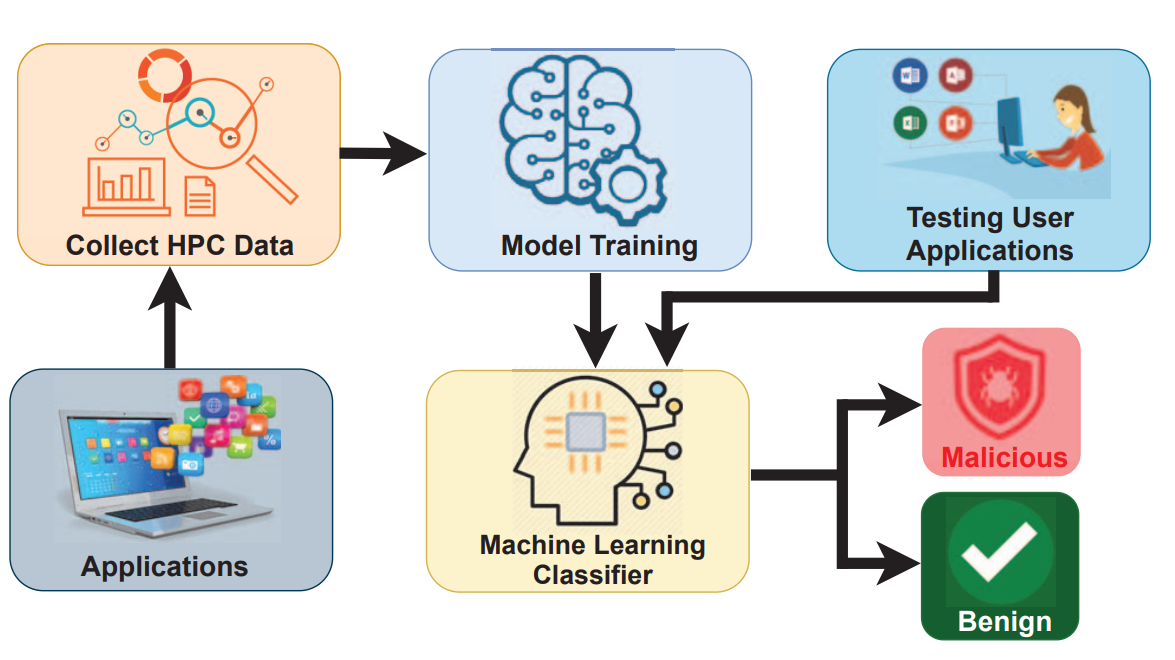
\includegraphics[width=\linewidth, height=150pt]{contents/images/time_series_1.png}
    \caption{An overview of HMDs \cite{time_series}}
    \label{fig:time_series_1}
\end{figure}

The reason for the necessity of the classification between benign and malicious programs is due to the large false-positive rate for HMDs. Imagine a situation where a heavily used application is marked as malicious, it would prevent users from adopting this HMD. 

As mentioned earlier the SEQ-TSD framework architecture is shown below:

\begin{figure}[h]
    \centering
    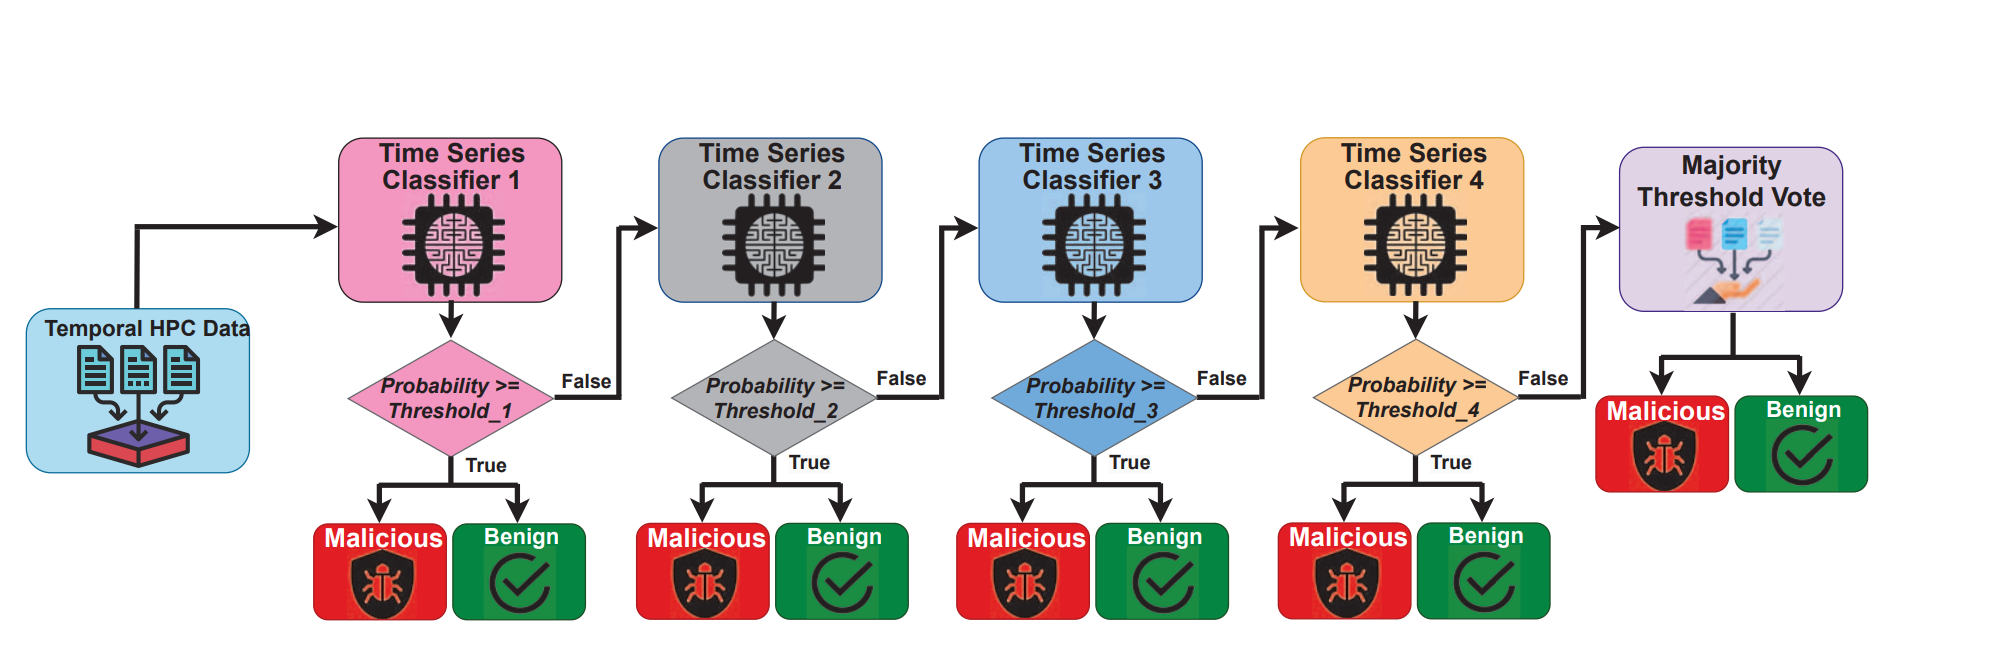
\includegraphics[width=\linewidth, height=100pt]{contents/images/time_series_2.png}
    \caption{Overview of the Proposed SEQ-TSD \cite{time_series}}
    \label{fig:time_series_2}
\end{figure}

The experiment consisted of getting a baseline of HPC readings using an Intel i5-4210u processor which uses the x86 Instruction Set Architecture (ISA) and then the same is done on an ARM Cortex-A53, the batches are 100 benign/malicious programs and 300 benign/malicious programs respectively. Below shows the accuracy of the varying time series length classifications for both the ARM and x86 Malware Datasets (AMD, XMD, respectively) \cite{time_series}:

\begin{figure}[h]
    \centering
    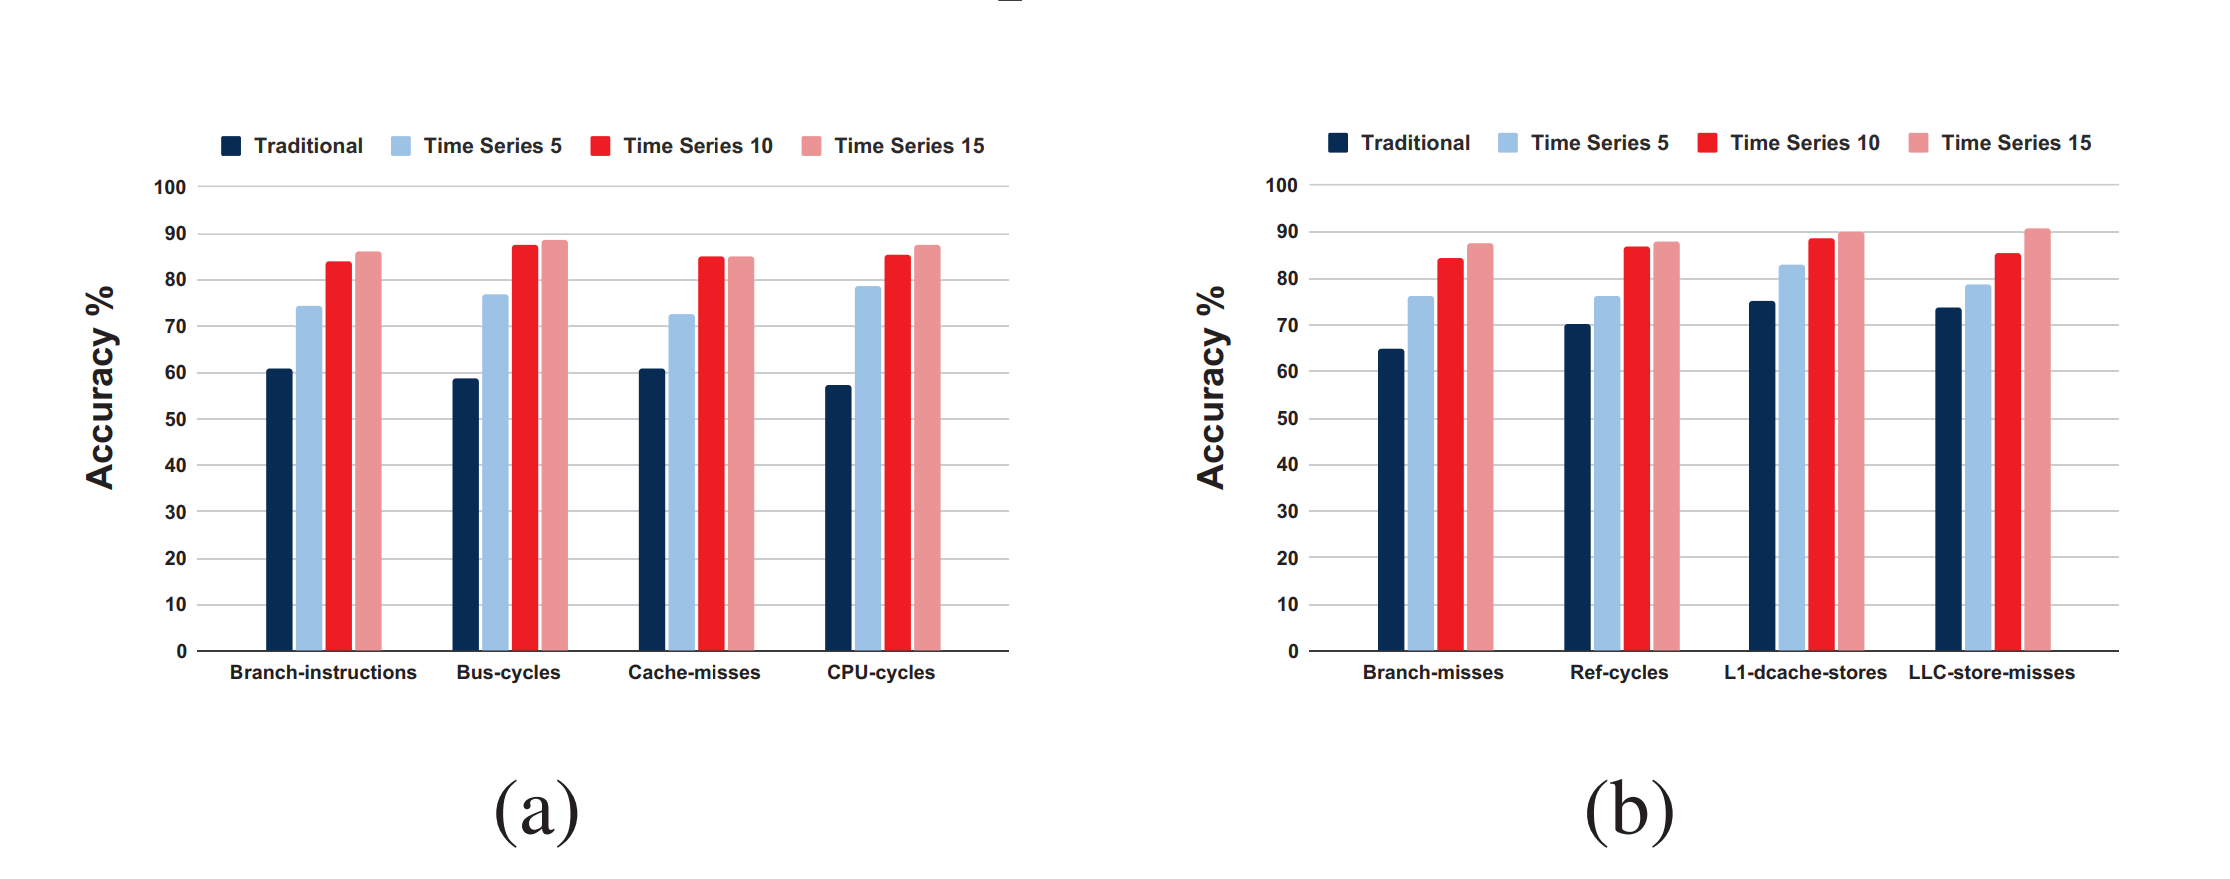
\includegraphics[width=200pt, height=100pt]{contents/images/time_series_3.png}
    \caption{(a) ARM Malware Dataset (AMD) and (b) x86 Malware Dataset (XMD)}
    \label{fig:time_series_3}
\end{figure}

And below the precision of the accompanying datasets \cite{time_series}:

\begin{figure}[h]
    \centering
    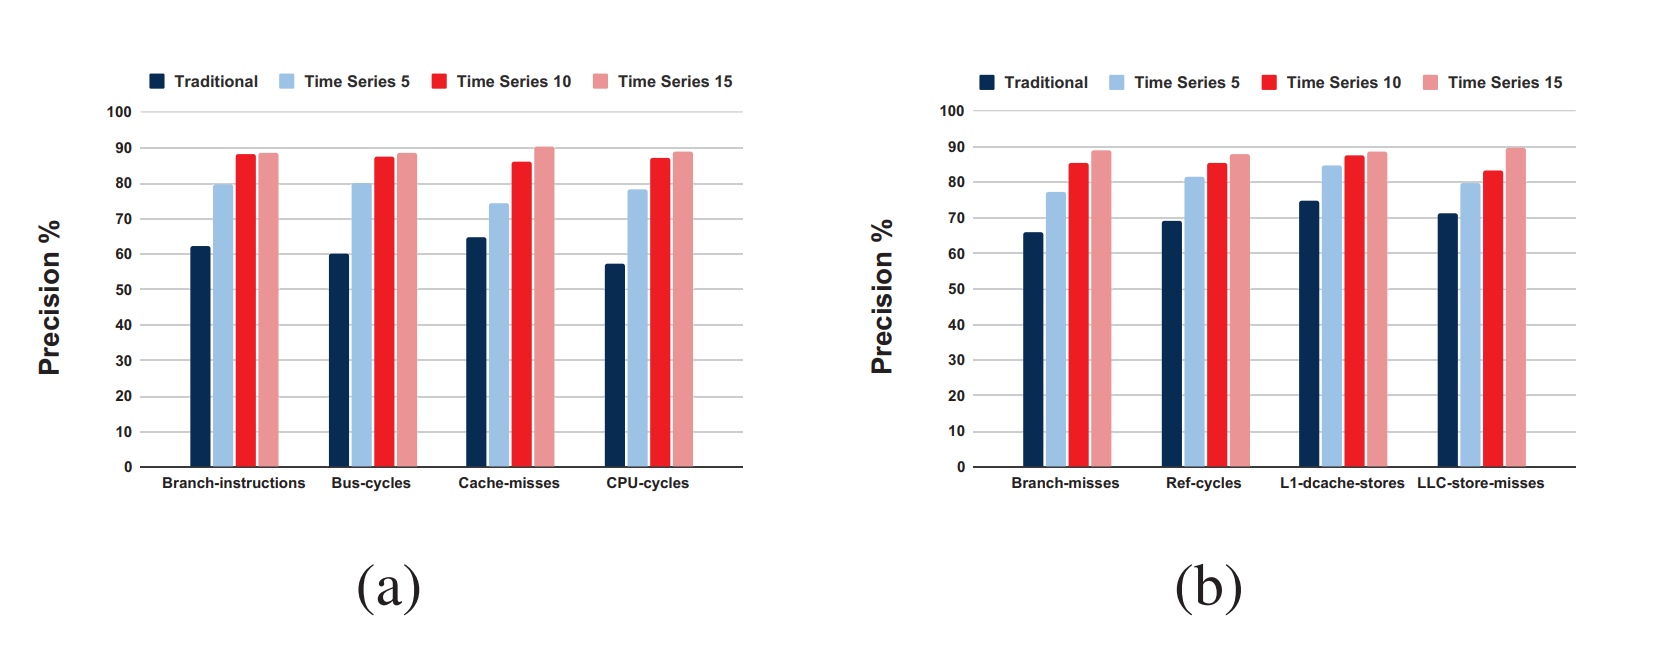
\includegraphics[width=200pt, height=100pt]{contents/images/time_series_4.png}
    \caption{(a) ARM Malware Dataset (AMD) and (b) x86 Malware Dataset (XMD)}
    \label{fig:time_series_4}
\end{figure}

As you can see adding a Time-Series classification leads to detection with a higher accuracy, lowering the false positive rate. Teh average improvement for AMD was around 16.21\% while it was 7.46\% for XMD for series length of 5. The average accuracy increases as the series length increases. 

Overall, although HMDs address the challenges of AVS, the high false-positive rate makes it less than ideal. The introduced Time Series Malware Detection (TSD) are clearly more advantageous than Traditional Malware Detection (TMD). The provided framework is able to produce detectors with 97.91\% accuracy with a flase-positive rate of 5.56\% using just a single HPC \cite{time_series}.

\end{document}